\documentclass[english, 11 pt, class=article, crop=false]{standalone}
%\documentclass[english, 11 pt]{report}
\usepackage[T1]{fontenc}
\usepackage[utf8]{luainputenc}
\usepackage{babel}
\usepackage[hidelinks, bookmarks]{hyperref}
\usepackage{geometry}
\geometry{verbose,tmargin=1cm,bmargin=3cm,lmargin=4cm,rmargin=4cm,headheight=3cm,headsep=1cm,footskip=1cm}
\setlength{\parindent}{0bp}
\usepackage{amsmath}
\usepackage{amssymb}
\usepackage{esint}
\usepackage{import}
\usepackage[subpreambles=false]{standalone}
%\makeatletter
\addto\captionsenglish{\renewcommand{\chaptername}{Kapittel}}
\makeatother
\usepackage{tocloft}
\addto\captionsenglish{\renewcommand{\contentsname}{Innhold}}
\usepackage{graphicx}
\usepackage{placeins}
\raggedbottom
\usepackage{calc}
\usepackage{cancel}
\makeatletter
\usepackage{color}
\definecolor{shadecolor}{rgb}{0.105469, 0.613281, 1}
\usepackage{framed}
\usepackage{wrapfig}
\usepackage{bm}
\usepackage{ntheorem}

\usepackage{ragged2e}
\RaggedRight
\raggedbottom
\frenchspacing

\newcounter{lign}[section]
\newenvironment{lign}[1][]{\Large \refstepcounter{lign} \large
	\textbf{\thelign #1} \rmfamily}{\par\medskip}
\numberwithin{lign}{section}
\numberwithin{equation}{section}
\usepackage{xcolor}
\usepackage{icomma}
\usepackage{mathtools}
\usepackage{lmodern} % load a font with all the characters
\usepackage{xr-hyper}
\makeatother
\usepackage[many]{tcolorbox}

%\setlength{\parskip}{\medskipamount}
\newcommand{\parskiplength}{11pt}
%\setlength{\parskip}{0 pt}
\newcommand\eks[2][]{\begin{tcolorbox}[enhanced jigsaw,boxrule=0.3 mm, arc=0mm,breakable,colback=green!30] {\large \textbf{Eksempel #1} \vspace{\parskiplength}\\} #2 \vspace{1pt} \end{tcolorbox}\vspace{1pt}}

\newcommand\fref[2][]{\hyperref[#2]{\textsl{Figur \ref*{#2}#1}}}
\newcommand{\hr}[2]{\hyperref[#2]{\color{blue}\textsl{#1}}}

\newcommand\rgg[2][]{\begin{tcolorbox}[boxrule=0.3 mm, arc=0mm,colback=orange!55] #2 \vspace{1pt} \end{tcolorbox}\vspace{-2pt}}
\newcommand\alg[1]{\begin{align*} #1 \end{align*}}
\newcommand\algv[1]{\vspace{-11 pt} \begin{align*} #1 \end{align*}}
\newcommand\vs{\vspace{-11 pt}}
\newcommand\g[1]{\begin{center} {\tt #1}  \end{center}}
\newcommand\gv[1]{\begin{center} \vspace{-22 pt} {\tt #1} \vspace{-11 pt} \end{center}}
%\addto\captionsenglish{\renewcommand{\contentsname}{Løsningsforslag tentamen R2 H2015}}

% Farger
\colorlet{shadecolor}{blue!30} 

% Figur
\usepackage{float}
\usepackage{subfig}
\captionsetup[subfigure]{labelformat=empty}
\usepackage{esvect}

\newcommand\sv{\textbf{Svar:} \vspace{5 pt} \\}

%Tableofconents
\renewcommand{\cfttoctitlefont}{\Large\bfseries}
\setlength{\cftsubsecindent}{2 cm}
\newcommand\tocskip{6 pt}
\setlength{\cftaftertoctitleskip}{30 pt}
\setlength{\cftbeforesecskip}{\tocskip}
%\setlength{\cftbeforesubsecskip}{\tocskip}

%Footnote:
\usepackage[bottom, hang, flushmargin]{footmisc}
\usepackage{perpage} 
\MakePerPage{footnote}
\addtolength{\footnotesep}{2mm}
\renewcommand{\thefootnote}{\arabic{footnote}}
\renewcommand\footnoterule{\rule{\linewidth}{0.4pt}}

%asin, atan, acos
\DeclareMathOperator{\atan}{atan}
\DeclareMathOperator{\acos}{acos}
\DeclareMathOperator{\asin}{asin}

%Tabell
\addto\captionsenglish{\renewcommand{\tablename}{Figur}}

% Figur
\usepackage[font=footnotesize,labelfont=sl]{caption}
\addto\captionsenglish{\renewcommand{\figurename}{Figur}}

% Figurer
\newcommand\scr[1]{/home/sindre/R/scr/#1}
\newcommand\asym[1]{/home/sindre/R/asymptote/#1}

%Toc for seksjoner
\newcommand\tsec[1]{\phantomsection\addcontentsline{toc}{section}{#1}
	\section*{#1}}
%\newcommand\tssec[1]{\subsection*{#1}\addcontentsline{toc}{subsection}{#1}}
\newcommand\tssec[1]{\subsection*{#1}}
% GeoGebra
\newcommand{\cms}[2]{{\tt #1( #2 )}}
\newcommand{\cm}[2]{{\large \tt #1( #2 )} \gvs \\}
\newcommand{\cmc}[2]{{\large \tt #1( #2 )} \large (CAS)  \gvs \\ \normalsize}
\newcommand{\cmk}[2]{{\large \tt #1( #2 )} \large (Inntastingsfelt)  \gvs \\ \normalsize}

\newcommand\gvs{\vspace{11 pt}}

\newcommand\vsk{\vspace{11 pt}}
\newcommand{\merk}{\vsk \textsl{Merk}: }
\newcommand{\fig}[1]{
\begin{figure}
	\centering
	\includegraphics[scale=0.5]{fig/#1}
\end{figure}
}
\newcommand{\figc}[1]{
		\centering
		\includegraphics[scale=0.5]{fig/#1}
}

% Opg
%\newcommand{\opgt}{\phantomsection \addcontentsline{toc}{section}{Oppgaver} \section*{Oppgaver for kapittel \thechapter}}
\newcounter{opg}
\numberwithin{opg}{section}

\newcommand{\opl}[1]{\vspace{15pt} \refstepcounter{opg} \textbf{\theopg} \vspace{2 pt} \label{#1} \\}



\begin{document}
\subimport{/home/sindre/R/ggb/}{ncmd}

\tsec{Knapper}
\renewcommand{\arraystretch}{1.5}	
\subsection*{Grafikkfelt}
Knappene velges fra rullemenyer på verktøylinjen. Nummereringen av menyene er fra venstre.\vsk

\begin{tabular}{@{}l}
	\,
\includegraphics[scale=0.4]{fig/pkt} Lager et nytt punkt. (Meny nr. 1) \\
	\,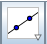
\includegraphics[scale=0.4]{fig/lin} Lager linje mellom to punkt. (Meny nr. 2)\\	
	\,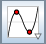
\includegraphics[scale=0.4]{fig/ekst} Finner topp- og bunnpunkt til en funksjon. (Meny nr. 2)\\
	\,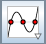
\includegraphics[scale=0.4]{fig/nul} Finner nullpunktene til en funksjon. (Meny nr. 2)	\\
	\,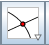
\includegraphics[scale=0.4]{fig/skj} Finner skjæringspunkt mellom to objekt. (Meny nr. 3)\\	
	\,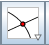
\includegraphics[scale=0.4]{fig/skj} Lager vektoren mellom to punkt (Meny nr. 3)\\		
	\,
\includegraphics[scale=0.4]{fig/tekst} Lager en tekstboks. (Meny nr. 10)\\		
	\,
\includegraphics[scale=0.4]{fig/flytt} Flytter grafikkfeltet. Endrer verdiavstanden hvis man peker på aksene. (Meny nr. 10)\\			
\end{tabular}
\subsection*{CAS}
\begin{tabular}{@{}l}
	\;
\includegraphics[scale=0.4]{fig/erlik} Gjengir uttrykket som er inntastet, ofte i forkortet form.\\	
	\;
\includegraphics[scale=0.4]{fig/brin} Gjengir uttrykket som er inntastet.\\	
	\;
\includegraphics[scale=0.4]{fig/caerlik} Gir tilnærmet verdi av et uttrykk (som desimaltall). \\	
	\;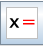
\includegraphics[scale=0.4]{fig/x} Gir eksaktløsningen av en ligning.\\
	\;
\includegraphics[scale=0.4]{fig/xca} Gir tilnærmet løsning av en ligning som desimaltall.\\

\end{tabular}

\tsec{Hurtigtaster}
\begin{tabular}{@{}c | c |c | c }
	&\textbf{Beskrivelse} & \textbf{PC }& \textbf{Mac} \\ \hline
	$ \sqrt{} $	& kvadratrot& \texttt{alt\,+\,r} &\texttt{alt\,+\,r} \\\hline
	$ \pi $	& pi& \texttt{alt\,+\,p} & \texttt{alt\,+\,p}\\\hline
	$ \infty $ &uendelig& \texttt{alt\,+\,u} &\texttt{alt\,+\,,}  \\\hline
	$ \otimes $&kryssprodukt & \texttt{alt\,+\,shift\,+\,8}&\texttt{ctrl\,+\,shift\,+\,8} \\\hline
	$ e $&eulers tall & \texttt{alt\,+\,e}& \texttt{alt\,+\,e}\\\hline
	$ {}^\circ $&gradtegnet ($ \frac{\pi}{180} $) & \texttt{alt\,+\,o}& \texttt{alt\,+\,o}
	\\\hline	
\end{tabular}

\tsec{Kommandoliste}\vs
\setlength{\parskip}{12 pt}
\renewcommand{\vsk}{\vspace{0 pt}}
\renewcommand\gvs{\vspace{1 pt}}
\cm{abs}{<x>}
Finner lengden til et objekt \textit{x}. (Merk: kan brukes til å finne lengden av en vektor).

\cm{Asymptote}{<Funksjon>}
Finner asymptotene til en funksjon.

\avst

\cmc{ByttUt}{<Uttrykk>, <Liste med forandringer>}
Viser et gitt uttrykk etter endring av variabler, gitt i en liste.

\der

\ekstpkt

\cm{Ekstremalpunkt}{Polynom}
Finner alle ekstremalpunkt og ekstremalverdier til et polynom.

\funk

\cmc{HøyreSide}{<Likning>}
Gir høyresiden til en likning.

\cmc{HøyreSide}{<Liste med likninger>}
Gir en liste med høyresidene i en liste med ligninger.

\intu

\intb

\cmc{Integral}{<Variabel>}
Gir uttrykket til det ubestemte integralet til en funksjon av gitt variabel. (Brukes dersom man ønsker å integrere funksjoner avhengig av en annen variabel enn $ x $).

\kurve

\kuler

\los

\cmc{Løs}{<Liste med likninger>, <Liste med variabler>}
Finner alle løsninger av en liste med ligninger med gitte variabel som ukjente.

\cmc{Løs}{<Likning>, <Variabel>}
Finner alle løsninger av en gitt likning med en gitt variabel som ukjent.

\dif

\diff

\absmaks

\absmin

\cm{Nullpunkt}{<Polynom> }
Finner alle nullpunkter til et polynom.

\cm{NullpunktIntervall}{<Funksjon>, <Start>, <Slutt>}
Finner alle nullpunkter på et gitt intervall til en hvilken som helst funksjon.

\plan

\pris

\punkt

\pyr

\cm{RegLin}{<Liste>}
Bruker regresjon med en rett linje for å tilpasse punkt gitt i en liste.

\cm{RegEksp}{<Liste>}
Bruker regresjon med en eksponentialfunksjon for å tilpasse punkt gitt i en liste.

\cm{RegPoly}{<Liste>, <Grad>}
Bruker regresjon med et polynom av gitt grad for å tilpasse punkt gitt i en liste.

\cm{RegPot}{<Liste>}
Bruker regresjon med en potensfunksjon for å tilpasse punkt gitt i en liste.

\regsin

\retn

\skalar

\cm{Skjæring}{<Objekt>, <Objekt>}
Finner skjæringspunktene mellom to objekter. 

\merk Fungerer ikke for vektorer, og gir bare ett av punktene dersom funksjonene har flere skjæringspunkt.

\cm{Skjæring}{<Funksjon>, <Funksjon>, <Start>, <Slutt>}
Finner skjæringspunktene mellom to funksjoner på et gitt intervall.

\summ

\cm{TrigKombiner}{<Funksjon>}
Skriver om et uttrykk på formen $ a\sin (kx) + b\cos (kx) $ til et kombinert uttrykk på formen $ r\cos (kx-c) $

\trikomb

\vektor

\vekpro

\vend

\cmc{VenstreSide}{<Likning>}
Gir venstresiden til en likning.

\cmc{VenstreSide}{<Liste med likninger>}
Gir en liste med venstresidene i en liste med ligninger.

\vink






\end{document}